
%(BEGIN_QUESTION)
% Copyright 2015, Tony R. Kuphaldt, released under the Creative Commons Attribution License (v 1.0)
% This means you may do almost anything with this work of mine, so long as you give me proper credit

Calculate all phase voltages and currents in the load given an open fault in one of the source's (alternator's) coils:

$$\includegraphics[width=15.5cm]{i02363x01.eps}$$

% No blank lines allowed between lines of an \halign structure!
% I use comments (%) instead, so that TeX doesn't choke.

$$\vbox{\offinterlineskip
\halign{\strut
\vrule \quad\hfil # \ \hfil & 
\vrule \quad\hfil # \ \hfil \vrule \cr
\noalign{\hrule}
%
% First row
{\bf Phase quantity} & {\bf Value} (volts/amps) \cr
%
\noalign{\hrule}
%
% Another row
$V_{R1}$ &  \cr
%
\noalign{\hrule}
%
% Another row
$V_{R2}$ &  \cr
%
\noalign{\hrule}
%
% Another row
$V_{R3}$ &  \cr
%
\noalign{\hrule}
%
% Another row
$I_{R1}$ &  \cr
%
\noalign{\hrule}
%
% Another row
$I_{R2}$ &  \cr
%
\noalign{\hrule}
%
% Another row
$I_{R3}$ &  \cr
%
\noalign{\hrule}
} % End of \halign 
}$$ % End of \vbox

\vfil

\underbar{file i02363}
\eject
%(END_QUESTION)





%(BEGIN_ANSWER)

This is a graded question -- no answers or hints given!

%(END_ANSWER)





%(BEGIN_NOTES)

With the failed-open winding in the three-phase generator, the load essentially sees nothing but 480 VAC across $R_3$, with $R_1$ and $R_2$ acting as a voltage divider dropping half of the 480 volts each.  The failure of that one phase coil in the three-phase source now means the load only receives a single sine wave between the two functioning power conductors.  In other words, this source fault has {\it ``single-phased''} the load.

\vskip 10pt

The equivalent circuit is shown here:

$$\includegraphics[width=15.5cm]{i02363x02.eps}$$

% No blank lines allowed between lines of an \halign structure!
% I use comments (%) instead, so that TeX doesn't choke.

$$\vbox{\offinterlineskip
\halign{\strut
\vrule \quad\hfil # \ \hfil & 
\vrule \quad\hfil # \ \hfil \vrule \cr
\noalign{\hrule}
%
% First row
{\bf Phase quantity} & {\bf Value} (volts/amps) \cr
%
\noalign{\hrule}
%
% Another row
$V_{R1}$ & 240 V \cr
%
\noalign{\hrule}
%
% Another row
$V_{R2}$ & 240 V \cr
%
\noalign{\hrule}
%
% Another row
$V_{R3}$ & 480 V \cr
%
\noalign{\hrule}
%
% Another row
$I_{R1}$ & 2.087 A \cr
%
\noalign{\hrule}
%
% Another row
$I_{R2}$ & 2.087 A \cr
%
\noalign{\hrule}
%
% Another row
$I_{R3}$ & 4.174 A \cr
%
\noalign{\hrule}
} % End of \halign 
}$$ % End of \vbox


%INDEX% Documentation, binary logic: converting ladder logic (relay) diagram to logic gate diagram

%(END_NOTES)


